\section{CInterpreter\-Startup  Class Reference}
\label{classCInterpreterStartup}\index{CInterpreterStartup@{CInterpreter\-Startup}}
{\tt \#include $<$CInterpreter\-Startup.h$>$}

Inheritance diagram for CInterpreter\-Startup::\begin{figure}[H]
\begin{center}
\leavevmode
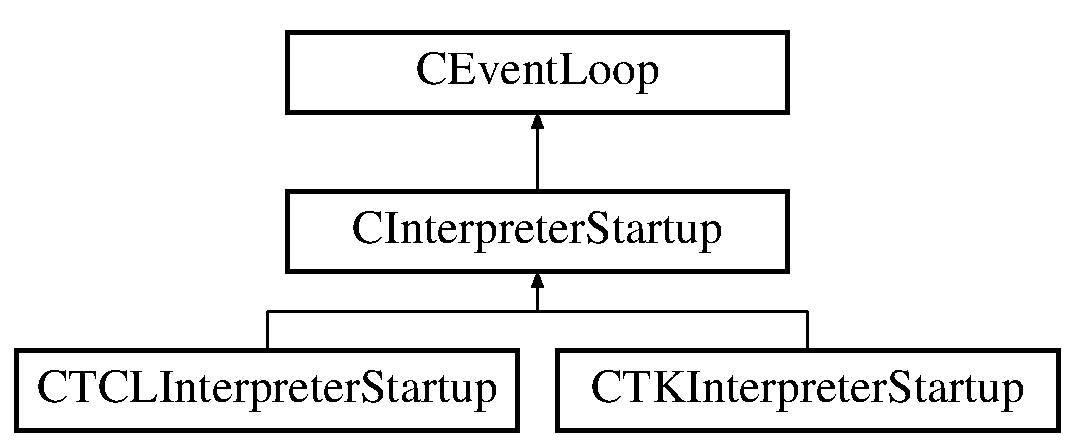
\includegraphics[height=3cm]{classCInterpreterStartup}
\end{center}
\end{figure}
\subsection*{Public Methods}
\begin{CompactItemize}
\item 
{\bf CInterpreter\-Startup} ()
\begin{CompactList}\small\item\em Nulls out the interpreter and sync command pointers.\item\end{CompactList}\item 
virtual {\bf $\sim$CInterpreter\-Startup} ()
\item 
{\bf CTCLInterpreter} $\ast$ {\bf get\-Interpreter} ()
\begin{CompactList}\small\item\em Return a pointer to the interpreter object.\item\end{CompactList}\item 
{\bf CTCLInterpreter} \& {\bf Interp} ()
\end{CompactItemize}
\subsection*{Protected Methods}
\begin{CompactItemize}
\item 
virtual void {\bf On\-Initialize} (int argc, char $\ast$$\ast$Argv)
\item 
virtual void {\bf Register\-Extensions} ()
\item 
void {\bf set\-Interpreter} ({\bf CTCLInterpreter} $\ast$p\-Interp)
\begin{CompactList}\small\item\em Set the interpreter object:.\item\end{CompactList}\end{CompactItemize}
\subsection*{Private Methods}
\begin{CompactItemize}
\item 
int {\bf operator()} (int argc, char $\ast$$\ast$argv)=0
\item 
{\bf CInterpreter\-Startup} (const CInterpreter\-Startup \&a\-CInterpreter\-Startup)
\begin{CompactList}\small\item\em Copy Constructor is forbidden, private, unimplemented.\item\end{CompactList}\item 
CInterpreter\-Startup \& {\bf operator=} (const CInterpreter\-Startup \&a\-CInterpreter\-Startup)
\begin{CompactList}\small\item\em Assignment is forbidden, private, unimplemented.\item\end{CompactList}\item 
int {\bf operator==} (const CInterpreter\-Startup \&a\-CInterpreter\-Startup) const
\begin{CompactList}\small\item\em Operator== Equality Operator forbidden, private, unimplemented.\item\end{CompactList}\end{CompactItemize}
\subsection*{Private Attributes}
\begin{CompactItemize}
\item 
{\bf CTCLInterpreter} $\ast$ {\bf m\_\-p\-Interp}
\item 
{\bf CTCLSynchronize\-Command} $\ast$ {\bf m\_\-p\-Sync\-Command}
\end{CompactItemize}


\subsection{Detailed Description}
Encapsulates interfaces for starting up  TCL based interpreter event loops. The TCL interpreter executes within a thread. Adding a command to the interpreter should be done by subclassing {\bf CDAQTCLProcessor} {\rm (p.\,\pageref{classCDAQTCLProcessor})}, instantiating an object for that class, and registring it on the current interpreter. It is important that DAQTCLProcessor objects be used rather than TCLProcessor objects since DAQTCLProcessor is thread-aware and will therefore synchronize its action through the application's global mutex. 



Definition at line 315 of file CInterpreter\-Startup.h.

\subsection{Constructor \& Destructor Documentation}
\index{CInterpreterStartup@{CInterpreter\-Startup}!CInterpreterStartup@{CInterpreterStartup}}
\index{CInterpreterStartup@{CInterpreterStartup}!CInterpreterStartup@{CInterpreter\-Startup}}
\subsubsection{\setlength{\rightskip}{0pt plus 5cm}CInterpreter\-Startup::CInterpreter\-Startup ()}\label{classCInterpreterStartup_a0}


Nulls out the interpreter and sync command pointers.

Encapsulates interfaces for starting up  TCL based interpreter event loops. The TCL interpreter executes within a thread. Adding a command to the interpreter should be done by subclassing {\bf CDAQTCLProcessor} {\rm (p.\,\pageref{classCDAQTCLProcessor})}, instantiating an object for that class, and registring it on the current interpreter. It is important that DAQTCLProcessor objects be used rather than TCLProcessor objects since DAQTCLProcessor is thread-aware and will therefore synchronize its action  through the application's global mutex. 

Definition at line 300 of file CInterpreter\-Startup.cpp.\index{CInterpreterStartup@{CInterpreter\-Startup}!~CInterpreterStartup@{$\sim$CInterpreterStartup}}
\index{~CInterpreterStartup@{$\sim$CInterpreterStartup}!CInterpreterStartup@{CInterpreter\-Startup}}
\subsubsection{\setlength{\rightskip}{0pt plus 5cm}CInterpreter\-Startup::$\sim$CInterpreter\-Startup ()\hspace{0.3cm}{\tt  [virtual]}}\label{classCInterpreterStartup_a1}


The destructor only destroys the sync command. The subclass is responsible for destroying the interpreter which in turn will unregister the sync command 

Definition at line 311 of file CInterpreter\-Startup.cpp.

References m\_\-p\-Sync\-Command.\index{CInterpreterStartup@{CInterpreter\-Startup}!CInterpreterStartup@{CInterpreterStartup}}
\index{CInterpreterStartup@{CInterpreterStartup}!CInterpreterStartup@{CInterpreter\-Startup}}
\subsubsection{\setlength{\rightskip}{0pt plus 5cm}CInterpreter\-Startup::CInterpreter\-Startup (const CInterpreter\-Startup \& {\em a\-CInterpreter\-Startup})\hspace{0.3cm}{\tt  [private]}}\label{classCInterpreterStartup_c1}


Copy Constructor is forbidden, private, unimplemented.



\subsection{Member Function Documentation}
\index{CInterpreterStartup@{CInterpreter\-Startup}!getInterpreter@{getInterpreter}}
\index{getInterpreter@{getInterpreter}!CInterpreterStartup@{CInterpreter\-Startup}}
\subsubsection{\setlength{\rightskip}{0pt plus 5cm}{\bf CTCLInterpreter}$\ast$ CInterpreter\-Startup::get\-Interpreter ()\hspace{0.3cm}{\tt  [inline]}}\label{classCInterpreterStartup_a2}


Return a pointer to the interpreter object.



Definition at line 353 of file CInterpreter\-Startup.h.\index{CInterpreterStartup@{CInterpreter\-Startup}!Interp@{Interp}}
\index{Interp@{Interp}!CInterpreterStartup@{CInterpreter\-Startup}}
\subsubsection{\setlength{\rightskip}{0pt plus 5cm}{\bf CTCLInterpreter}\& CInterpreter\-Startup::Interp ()\hspace{0.3cm}{\tt  [inline]}}\label{classCInterpreterStartup_a3}


Get a reference to the interpreter object: Note that this can fail if there is not yet an interpreter (m\_\-p\-Interp is NULL in that case). 

Definition at line 360 of file CInterpreter\-Startup.h.\index{CInterpreterStartup@{CInterpreter\-Startup}!OnInitialize@{OnInitialize}}
\index{OnInitialize@{OnInitialize}!CInterpreterStartup@{CInterpreter\-Startup}}
\subsubsection{\setlength{\rightskip}{0pt plus 5cm}void CInterpreter\-Startup::On\-Initialize (int {\em argc}, char $\ast$$\ast$ {\em Argv})\hspace{0.3cm}{\tt  [protected, virtual]}}\label{classCInterpreterStartup_b0}


On initialize is called very early in  the execution of the operator() member. It is intended that subclassed interpreters perform early initialization here. At this point an interpreter has not yet been  instantiated. Therefore, you may not perform Tcl/Tk library calls at this  stage.

Default implementation is a no-op. 

Definition at line 332 of file CInterpreter\-Startup.cpp.

Referenced by CTKInterpreter\-Startup::operator()(), and CTCLInterpreter\-Startup::operator()().\index{CInterpreterStartup@{CInterpreter\-Startup}!operator()@{operator()}}
\index{operator()@{operator()}!CInterpreterStartup@{CInterpreter\-Startup}}
\subsubsection{\setlength{\rightskip}{0pt plus 5cm}int CInterpreter\-Startup::operator() (int {\em argc}, char $\ast$$\ast$ {\em argv})\hspace{0.3cm}{\tt  [private, pure virtual]}}\label{classCInterpreterStartup_c0}


This pure virtual member function is expected to start the interpreter and call the other member functions; it is the entry point of the thread. 

Implements {\bf CEvent\-Loop} {\rm (p.\,\pageref{classCEventLoop_c0})}.

Implemented in {\bf CTCLInterpreter\-Startup} {\rm (p.\,\pageref{classCTCLInterpreterStartup_c0})}, and {\bf CTKInterpreter\-Startup} {\rm (p.\,\pageref{classCTKInterpreterStartup_c3})}.\index{CInterpreterStartup@{CInterpreter\-Startup}!operator=@{operator=}}
\index{operator=@{operator=}!CInterpreterStartup@{CInterpreter\-Startup}}
\subsubsection{\setlength{\rightskip}{0pt plus 5cm}CInterpreter\-Startup\& CInterpreter\-Startup::operator= (const CInterpreter\-Startup \& {\em a\-CInterpreter\-Startup})\hspace{0.3cm}{\tt  [private]}}\label{classCInterpreterStartup_c2}


Assignment is forbidden, private, unimplemented.

\index{CInterpreterStartup@{CInterpreter\-Startup}!operator==@{operator==}}
\index{operator==@{operator==}!CInterpreterStartup@{CInterpreter\-Startup}}
\subsubsection{\setlength{\rightskip}{0pt plus 5cm}int CInterpreter\-Startup::operator== (const CInterpreter\-Startup \& {\em a\-CInterpreter\-Startup}) const\hspace{0.3cm}{\tt  [private]}}\label{classCInterpreterStartup_c3}


Operator== Equality Operator forbidden, private, unimplemented.

\index{CInterpreterStartup@{CInterpreter\-Startup}!RegisterExtensions@{RegisterExtensions}}
\index{RegisterExtensions@{RegisterExtensions}!CInterpreterStartup@{CInterpreter\-Startup}}
\subsubsection{\setlength{\rightskip}{0pt plus 5cm}void CInterpreter\-Startup::Register\-Extensions ()\hspace{0.3cm}{\tt  [protected, virtual]}}\label{classCInterpreterStartup_b1}


Concrete subclasses of this class must implement this function. It is expected that all tcl interpreters run in this envrionment will have extensions At this point, an interpreter has been created.

If this is a Tk derived  interpreter, it's not certain that the tk Main window has been created yet however.

Default behavior which should be chained to by subclasses is to register the synch command. This makes available scripts which are synchronized to the application's global mutex. 

Definition at line 355 of file CInterpreter\-Startup.cpp.

References m\_\-p\-Interp, m\_\-p\-Sync\-Command, and CDAQTCLProcessor::Register().

Referenced by CTCLInterpreter\-Startup::Tcl\_\-Init(), and CTKInterpreter\-Startup::Tk\_\-Init().\index{CInterpreterStartup@{CInterpreter\-Startup}!setInterpreter@{setInterpreter}}
\index{setInterpreter@{setInterpreter}!CInterpreterStartup@{CInterpreter\-Startup}}
\subsubsection{\setlength{\rightskip}{0pt plus 5cm}void CInterpreter\-Startup::set\-Interpreter ({\bf CTCLInterpreter} $\ast$ {\em p\-Interp})\hspace{0.3cm}{\tt  [inline, protected]}}\label{classCInterpreterStartup_b2}


Set the interpreter object:.



Definition at line 368 of file CInterpreter\-Startup.h.

Referenced by CTCLInterpreter\-Startup::Tcl\_\-Init(), and CTKInterpreter\-Startup::Tk\_\-Init().

\subsection{Member Data Documentation}
\index{CInterpreterStartup@{CInterpreter\-Startup}!m_pInterp@{m\_\-pInterp}}
\index{m_pInterp@{m\_\-pInterp}!CInterpreterStartup@{CInterpreter\-Startup}}
\subsubsection{\setlength{\rightskip}{0pt plus 5cm}{\bf CTCLInterpreter}$\ast$ CInterpreter\-Startup::m\_\-p\-Interp\hspace{0.3cm}{\tt  [private]}}\label{classCInterpreterStartup_o0}




Definition at line 318 of file CInterpreter\-Startup.h.

Referenced by Register\-Extensions().\index{CInterpreterStartup@{CInterpreter\-Startup}!m_pSyncCommand@{m\_\-pSyncCommand}}
\index{m_pSyncCommand@{m\_\-pSyncCommand}!CInterpreterStartup@{CInterpreter\-Startup}}
\subsubsection{\setlength{\rightskip}{0pt plus 5cm}{\bf CTCLSynchronize\-Command}$\ast$ CInterpreter\-Startup::m\_\-p\-Sync\-Command\hspace{0.3cm}{\tt  [private]}}\label{classCInterpreterStartup_o1}




Definition at line 319 of file CInterpreter\-Startup.h.

Referenced by Register\-Extensions(), and $\sim$CInterpreter\-Startup().

The documentation for this class was generated from the following files:\begin{CompactItemize}
\item 
{\bf CInterpreter\-Startup.h}\item 
{\bf CInterpreter\-Startup.cpp}\end{CompactItemize}
